\section{RC4}

	\begin{frame}
		\begin{center}
			\LARGE{\textcolor{blue}{Dai blocchi allo stream: RC4}}
		\end{center}
	\end{frame}

	\subsection{Stream}
	
		\begin{frame}
			\frametitle{Stream cipher}		
			\begin{itemize}
				\item I cifrari a blocchi codificano input producendo output \tblue{un blocco alla volta}
				\item I cifrari a stream codificano l'input \tblue{costantemente} producendo output di volta in volta
				\item Generalmente si codifica \tblue{un byte} alla volta
				\item Necessita di un generatore di byte \tblue{pseudocasuali}
			\end{itemize}
		\end{frame}
	
		\begin{frame}
		\frametitle{Generatore pseudo-casuale}		
		\begin{itemize}
			\item Riceve in input la chiave e restituisce uno \tblue{stream} di byte pseudocasuali chiamato \tblue{keystream}
			\item Il keystream deve essere \tblue{impredicibile} senza conoscere la chiave
			\item Viene messo in XOR \tblue{bit a bit} con lo stream da cifrare
			\item Se lo stream fosse \tblue{veramente} casuale, otterremmo una sorta di One Time Pad
		\end{itemize}
	\end{frame}

	\subsection{RC4}
	
		\begin{frame}
			\frametitle{RC4}		
			\begin{itemize}
				\item Progettato nel 1987 da \tblue{Ron Rivest} per la RSA security
				\item Inizialmente la NSA lo aveva tenuto segreto ma fu diffuso anonimamente su internet nel \tblue{1994}
				\item Codifica \tblue{un byte} alla volta
				\item Il \tblue{periodo} del generatore pseudo-casuale è $\approx 10^{100}$
				\item Molto \tblue{veloce} (minimo 8 massimo 16 operazioni macchina per byte)
				\item Usato in SSL/TLS, lo \tblue{standard di comunicazione} tra browser e server
			\end{itemize}
		\end{frame}
	
		\begin{frame}
			\frametitle{Algoritmo}		
			\begin{itemize}
				\item Chiave a \tblue{lunghezza variabile}, da 1 a 256 bytes
				\item Con la chiave si inizializza il vettore di stato \tblue{S} di 256 bytes
				\item $S\left[ 0\right] , S\left[ 1\right] ,\dots,S\left[ 255\right] $ contengono una permutazione di \tblue{tutti} i numeri a 8 bit compresi tra 0 e 255
				\item Viene \tblue{scelto} un byte $S\left[ k\right] $ che viene usato per la encryption in modo sistematico
				\item Tutti i byte di S vengono \tblue{nuovamente permutati}
			\end{itemize}
		\end{frame}
	
		\begin{frame}
			\frametitle{Algoritmo}	
			\begin{columns}
				\begin{column}{0.65\textwidth}
					\begin{center}
						\begin{figure}
							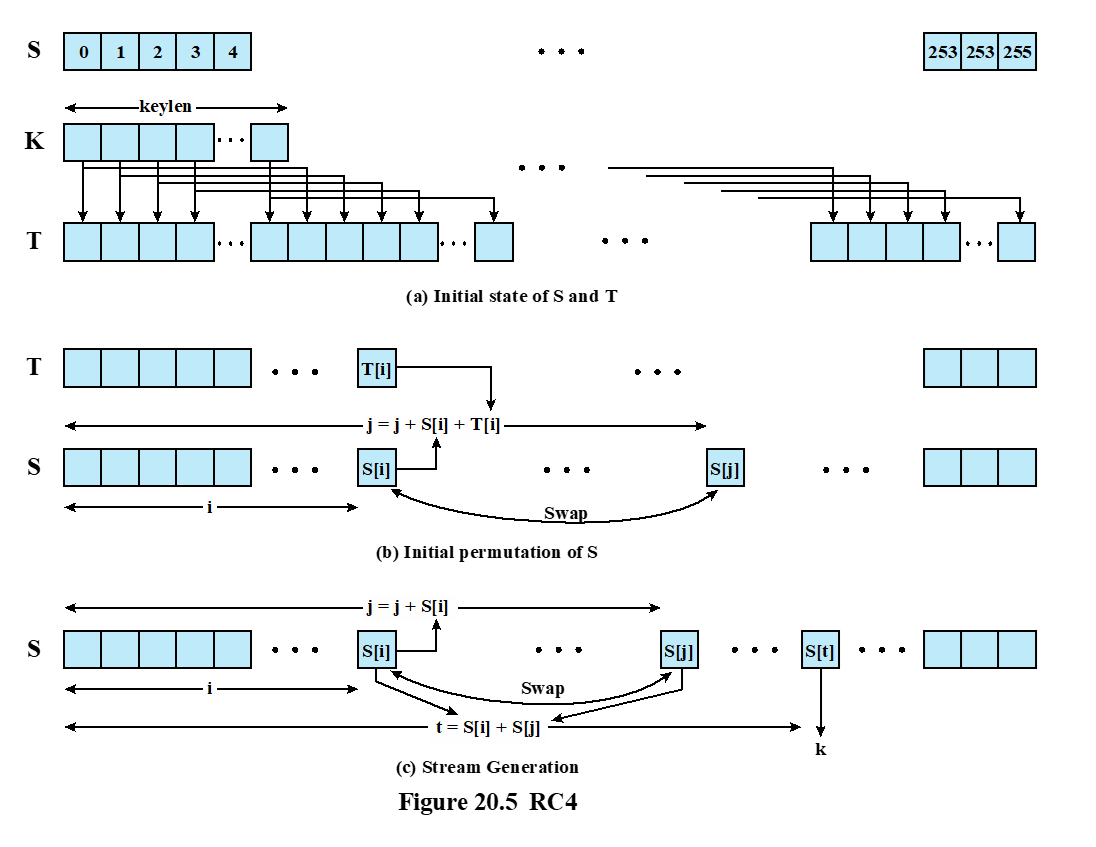
\includegraphics[width=\columnwidth]{img/rc4}
							\caption{Schema generale}
						\end{figure}
					\end{center}
				\end{column}
				\begin{column}{0.35\textwidth}
					\begin{center}
						\begin{figure}
							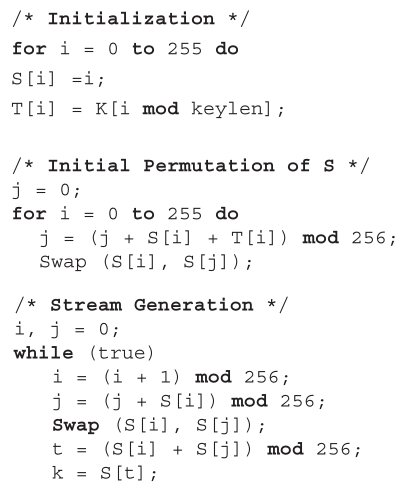
\includegraphics[width=\columnwidth]{img/rc4algo}
							\caption{Pseudocodice}
						\end{figure}
					\end{center}
				\end{column}
			\end{columns}	
		\end{frame}
	
	\subsection{Sicurezza}
		
		\begin{frame}
			\frametitle{(In)Sicurezza}	
			\begin{itemize}
				\item Molto semplice ma molto \tblue{debole}
				\item Il problema non è RC4 ma il \tblue{PRNG}
				\item Alta \tblue{periodicità} nei primi 256 bytes
				\item Forte \tblue{correlazione} tra chiave e keystream
			\end{itemize}
		\end{frame}
	
		\begin{frame}
			\frametitle{(In)Sicurezza}	
			\begin{itemize}
				\item Molte implementazioni eseguono un ciclo di 256 iterazioni \tblue{a vuoto} prima di utilizzare il keystream
				\item Mozilla \tblue{ha rimosso} da Firefox il supporto a RC4 dalla versione 44 (26 gennaio 2016)
				\item L'alternativa migliore attualmente è \tblue{SNOW} di Thomas Johansson e Patrik Ekdahl dell'università svedese di Lund
			\end{itemize}
		\end{frame}


